%% =====================================================================
%% Documento Final - EEE017 Confiabilidade de Sistemas
%% Trabalho final - UFMG (Prof. Michel Bessani)
%% Template: IEEEtran (conference)
%% Compilar com: pdflatex Documento_Final_EEE017.tex (executar duas vezes)
%% =====================================================================
\documentclass[conference]{IEEEtran}
\IEEEoverridecommandlockouts

% --- Pacotes essenciais ---------------------------------------------------
\usepackage[utf8]{inputenc}
\usepackage[T1]{fontenc}
\usepackage[brazil]{babel}
\usepackage{amsmath,amssymb,amsfonts}
\usepackage{graphicx}
\usepackage{cite}
\usepackage{url}
\usepackage{textcomp}
\usepackage{xcolor}
\usepackage{booktabs}
\usepackage{array}
\usepackage{tabularx}

% Empacotamento de floats: permite mais figuras por pagina e menos paginas
% so de figuras, eliminando os grandes espacos em branco. flushbottom (padrao
% do IEEEtran) preenche as colunas ate o fim.
\flushbottom
\renewcommand{\topfraction}{0.95}
\renewcommand{\bottomfraction}{0.9}
\renewcommand{\textfraction}{0.05}
\renewcommand{\floatpagefraction}{0.85}
\setcounter{topnumber}{3}
\setcounter{bottomnumber}{2}
\setcounter{totalnumber}{5}
\usepackage{hyperref}
\hypersetup{
    colorlinks=true,
    linkcolor=black,
    citecolor=black,
    urlcolor=blue
}

% Figuras geradas pelo pipeline em confiabilidade/code/resultados/figuras/
\graphicspath{{../code/resultados/figuras/}}

\def\BibTeX{{\rm B\kern-.05em{\sc i\kern-.025em b}\kern-.08em
    T\kern-.1667em\lower.7ex\hbox{E}\kern-.125emX}}

\begin{document}

% =========================================================================
% TITULO E AUTORES
% =========================================================================
\title{Análise de Confiabilidade de Bombas Centrífugas Industriais
       Acionadas por Motor Elétrico com Base em
       Dados Experimentais de Sensores de Vibração}

\author{
\IEEEauthorblockN{Felipe Costa Lopes}
\IEEEauthorblockA{\textit{UFMG} \\
Matrícula: 2018019648 \\
Belo Horizonte, MG, Brasil}
\and
\IEEEauthorblockN{Isabella Beatriz de Souza Gomes}
\IEEEauthorblockA{\textit{UFMG} \\
Matrícula: 2022421587 \\
Belo Horizonte, MG, Brasil}
\and
\IEEEauthorblockN{Stéphanie Pereira Barbosa}
\IEEEauthorblockA{\textit{UFMG} \\
Matrícula: 2021088965 \\
Belo Horizonte, MG, Brasil}
}

\maketitle

% =========================================================================
% RESUMO
% =========================================================================
\begin{abstract}
Este trabalho aplica métodos clássicos de Engenharia de Confiabilidade a um
conjunto motor-bomba centrífuga, usando o conjunto de dados experimental
público de Bruinsma \textit{et al.}~(2024), composto por medições de vibração e
corrente. Para os quatro modos de falha estudados (defeitos de rolamento, desbalanceamentos e desalinhamento),
utiliza-se exclusivamente o sinal de vibração. Como o conjunto de dados original é
composto por medições de condição (e não de vida até a falha), um indicador de degradação ---
o valor RMS da vibração em banda de frequência --- é extraído por modo de falha e usado para
calibrar um modelo de degradação exponencial. A partir dele, séries de tempo até a falha (TTF) com censura à
direita são geradas por simulação de Monte Carlo, sobre as quais se ajustam as
distribuições Exponencial, Weibull e Log-normal por máxima verossimilhança,
com seleção por AICc e intervalos de confiança por \textit{bootstrap}
($R=10^4$). Calculam-se MTTF, $R(t)$, taxa de falha $h(t)$ e disponibilidade
$A$ para quatro modos (rolamento, desbalanceamento no motor e na bomba e
desalinhamento). O conjunto é então modelado por Diagrama de Blocos de
Confiabilidade (motor em série com bomba) e simulado por Monte Carlo nas
configurações série, paralelo e \textit{standby}, com verificação analítica da
disponibilidade. Os parâmetros de forma obtidos ($\beta$ entre $0{,}98$ e
$3{,}82$) são coerentes com a literatura de desgaste de máquinas rotativas, e a
redundância eleva a disponibilidade de $\approx 0{,}98$ para $\approx 0{,}9997$.
\end{abstract}

\begin{IEEEkeywords}
Confiabilidade, bomba centrífuga, motor de indução, distribuição Weibull,
\textit{bootstrap}, Monte Carlo, monitoramento por vibração, manutenção.
\end{IEEEkeywords}

% =========================================================================
% I. INTRODUCAO
% =========================================================================
\section{Introdução}

A Engenharia de Confiabilidade estuda a probabilidade de um sistema executar
sua função, sob condições especificadas, durante um período de
tempo~\cite{oconnor2012}. Em plantas industriais, falhas não planejadas geram
paradas de produção e custos elevados, o que torna a estimativa de índices como
o Tempo Médio até a Falha (MTTF), a taxa de falha $\lambda(t)$ e a
disponibilidade $A$ central para a decisão de manutenção.

Bombas centrífugas acionadas por motores de indução estão entre os
equipamentos mais críticos da indústria. Seus principais modos de falha ---
defeitos de rolamento, desbalanceamento e desalinhamento --- têm
assinatura conhecida em sinais de vibração, o que motiva o uso
dessa técnica como base para a análise de confiabilidade baseada em
condição~\cite{bruinsma2024}.

O objetivo deste trabalho é responder, de forma reprodutível, a duas perguntas:
dado um modo de falha em desenvolvimento, qual a distribuição do tempo até a
falha funcional do equipamento? E quanto a configuração do sistema (uma unidade
ou com redundância) altera sua disponibilidade? Para isso aplicam-se a um
conjunto de dados experimental real os métodos da disciplina EEE017~\cite{bessani2026}: extração
de séries de TTF, ajuste de distribuições de vida com censura, \textit{bootstrap},
cálculo de índices e simulação de Monte Carlo de um Diagrama de Blocos de
Confiabilidade (DBC). Todo o código e os artefatos gerados são abertos e
acompanham este documento.

% =========================================================================
% II. REVISAO DA LITERATURA
% =========================================================================
\section{Revisão da Literatura}
\label{sec:revisao}

A análise estatística de dados de vida de equipamentos --- tempos até a falha
e dados censurados --- é tratada de forma abrangente em O'Connor e
Kleyner~\cite{oconnor2012} e Colosimo e Giolo~\cite{colosimo2006}. As
distribuições Weibull, Exponencial e Log-normal são as mais utilizadas em
confiabilidade de máquinas rotativas; o parâmetro de forma $\beta$ da Weibull é
particularmente valioso porque posiciona o equipamento na curva da banheira:
$\beta<1$ indica falhas prematuras, $\beta\approx 1$ taxa constante (vida útil),
e $\beta>1$ desgaste crescente~\cite{oconnor2012}.

Monitoramento por condição em conjuntos motor-bomba é um campo consolidado.
Bruinsma \textit{et al.}~\cite{bruinsma2024} demonstram que vibração e corrente são
as técnicas mais aplicadas para detecção precoce de defeitos. Neste trabalho,
o monitoramento foca na análise de vibração, na qual defeitos de rolamento
manifestam-se em banda de alta frequência (impactos em 1--9\,kHz), enquanto
desbalanceamento e desalinhamento dominam os harmônicos de baixa frequência
(1$\times$ e 2$\times$ a rotação), justificando a separação em bandas para
construção do indicador de degradação~\cite{bruinsma2024}.

A ponte entre dados de condição (\textit{snapshots}) e análise de confiabilidade
é abordada por Meeker e Escobar~\cite{meeker1998} via modelos de degradação: a
trajetória de deterioração é parametrizada e a distribuição da vida útil é
derivada analiticamente ou por simulação. Essa abordagem é especialmente
relevante quando não há dados de operação contínua até a falha, como no presente
estudo.

O método \textit{bootstrap} para intervalos de confiança em parâmetros de
distribuições de vida é apresentado por Robert e Casella~\cite{robert2010} e
é computacionalmente robusto mesmo com censura à direita. A modelagem de sistemas
por Diagrama de Blocos de Confiabilidade e a avaliação de cenários de redundância
por Monte Carlo são fundamentadas em Zio~\cite{zio2013}.

% =========================================================================
% III. SISTEMA E DADOS
% =========================================================================
\section{Sistema e Dados}
\label{sec:dados}

\subsection{Conjunto de Dados}
Utiliza-se o \textit{Motor Current and Vibration Monitoring Dataset for various
Faults in an E-motor-driven Centrifugal Pump}~\cite{bruinsma2024}, coletado no
\textit{Fieldlab Techport} pela Marinha Real dos Países Baixos em parceria com a
Universidade de Twente, e disponível publicamente (licença CC0). O sistema
físico é um conjunto motor de indução + bomba centrífuga NK80, instrumentado
com cinco acelerômetros (Wilcoxon 786B-10, 100\,mV/g) e medição trifásica de
corrente e tensão, todos amostrados a 20\,kHz.

O conjunto registra a condição saudável e falhas induzidas em vários níveis de
severidade: defeitos de rolamento (pistas interna e externa, BPFI/BPFO),
desbalanceamento no motor e na bomba, desalinhamento angular e paralelo,
cavitação e dano no impelidor. Cada arquivo CSV contém a coluna de tempo e
diversas colunas, em que cada coluna é uma \textit{repetição independente} da
mesma medição (até 55 repetições na vibração).

\subsection{Natureza dos Dados e Implicação Metodológica}
É essencial observar que o conjunto é de medições de condição
(\textit{snapshots}), e não de operação contínua até a falha
(\textit{run-to-failure}). Não existe, portanto, um eixo de tempo real de
degradação. A ponte para a análise de confiabilidade, descrita na
Seção~\ref{sec:metodo}, trata os níveis de severidade como instantes de uma
trajetória de degradação e gera os tempos até a falha por um modelo calibrado
nos dados, segundo a abordagem de confiabilidade por degradação de Meeker e
Escobar~\cite{meeker1998}.

% =========================================================================
% III. MATERIAIS E METODOS
% =========================================================================
\section{Materiais e Métodos}
\label{sec:metodo}

A metodologia tem seis etapas, implementadas em Python (bibliotecas
\texttt{numpy}, \texttt{scipy}, \texttt{pandas} e
\texttt{reliability}~\cite{reid2022}).

\subsection{Indicador de Degradação}
Para cada modo de falha computa-se, em cada repetição, o valor RMS do sinal de
vibração em uma banda de frequência, obtido pela densidade espectral de Welch:
\begin{equation}
\mathrm{RMS}_{banda} = \sqrt{\int_{f_1}^{f_2} S_{xx}(f)\,df}.
\end{equation}
A banda é escolhida pela física da falha e validada por correlação de Spearman
com a severidade: banda alta (1--9\,kHz) para rolamento, onde aparecem
os impactos de alta frequência, e banda baixa (10--300\,Hz) para
desbalanceamento e desalinhamento, dominados pelos harmônicos $1\times$ e
$2\times$ da rotação. O RMS de banda larga puro não distingue defeitos de
rolamento da condição saudável, o que justifica a separação por banda. A
Fig.~\ref{fig:assinatura} mostra a assinatura resultante: o indicador cresce
de forma monotônica do estado saudável até a severidade máxima.

\begin{figure}[!t]
  \centering
  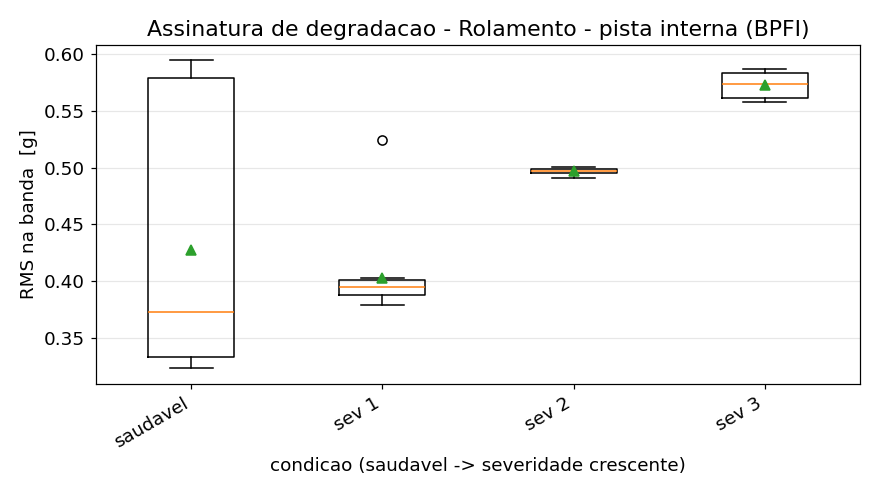
\includegraphics[width=\columnwidth]{p1_assinatura_bpfi.png}
  \caption{Indicador de degradação (RMS de vibração em banda) por nível de
  severidade, para o rolamento BPFI. A caixa do estado saudável é larga
  (variabilidade entre medições de referência) e as severidades crescem de
  forma ordenada.}
  \label{fig:assinatura}
\end{figure}

\subsection{Construção das Séries de TTF}
Modela-se a degradação como crescimento exponencial
$D(\tau)=D_0\,e^{\rho\tau}$, em que $\tau$ é o tempo de operação acumulada. Cada
nível de severidade $s$ é mapeado em $\tau_s = s\cdot\Delta\tau$, com
$\Delta\tau=1000$~h (premissa de escala, discutida na Seção~\ref{sec:disc}). A
taxa média $\bar\rho$ é calibrada nos dados, do estado saudável até a severidade
máxima. Cada unidade simulada recebe uma taxa aleatória
$\rho = \bar\rho\cdot e^{\mathcal{N}(0,\,c)}$, com $c=0{,}4$, que representa a
variabilidade operacional unidade-a-unidade que um conjunto de \textit{snapshots}
não fornece. A falha ocorre quando $D$ cruza o limiar
$L = \mu_0 + 0{,}5\,(D_{max}-\mu_0)$, inspirado nas zonas de alarme da
ISO~20816-3~\cite{iso20816}. Unidades que não cruzam $L$ até o horizonte são
censuradas à direita. Geram-se 2000 unidades por modo.

\subsection{Ajuste de Distribuições e Seleção}
Sobre as TTF (falhas e censuras) ajustam-se as distribuições Exponencial,
Weibull-2P e Log-normal por máxima verossimilhança com censura à
direita~\cite{colosimo2006}. Para a Weibull,
\begin{equation}
\log L(\beta,\eta) = \!\!\sum_{i\in O}\!\log f(t_i;\beta,\eta)
                   + \!\!\sum_{j\in C}\!\log R(t_j;\beta,\eta),
\end{equation}
com $f(t)=(\beta/\eta)(t/\eta)^{\beta-1}e^{-(t/\eta)^\beta}$ e
$R(t)=e^{-(t/\eta)^\beta}$, sendo $O$ as falhas e $C$ as censuras. A escolha
entre distribuições usa o AICc, e a aderência é verificada por
Kolmogorov--Smirnov. Os pontos empíricos dos gráficos usam os \textit{median
ranks} de Benard, $r_i=(i-0{,}3)/(n+0{,}4)$.

\subsection{Intervalos de Confiança por Bootstrap}
Para os parâmetros da Weibull ($\beta$, $\eta$), constroem-se intervalos de 95\%
por \textit{bootstrap} não paramétrico com $R=10^4$ reamostragens com reposição
dos pares $(t,\text{censura})$, reajustando a distribuição a cada
reamostra~\cite{robert2010}.

\subsection{Índices de Confiabilidade}
Da distribuição vencedora obtêm-se: $\mathrm{MTTF}=\int_0^\infty R(t)\,dt$, a
confiabilidade $R(t)$, a taxa de falha $h(t)=f(t)/R(t)$ e a disponibilidade
$A=\mathrm{MTTF}/(\mathrm{MTTF}+\mathrm{MTTR})$, com $\mathrm{MTTR}=24$~h. O
parâmetro de forma $\beta$ da Weibull indica o estágio na curva da banheira.

\subsection{Modelo de Sistema e Monte Carlo}
O conjunto é um DBC com o motor em série com a bomba (a falha de qualquer um
para o conjunto). Por inversão da CDF, $t=F^{-1}(U)$ com $U\sim\mathcal{U}(0,1)$,
simulam-se $N=10^5$ tempos de falha e avaliam-se três configurações: série (uma
unidade, arranjo real), paralelo (duas unidades ativas, basta uma) e
\textit{standby} (reserva acionada após a falha da primeira). As expressões
analíticas $A_{s}=\prod_i A_i$, $A_{p}=1-\prod_i(1-A_i)$ e
$A_{sb}=(\mu^2+\mu\lambda)/(\mu^2+\mu\lambda+\lambda^2)$ verificam a
simulação~\cite{zio2013}.

% =========================================================================
% IV. RESULTADOS
% =========================================================================
\section{Resultados}

Foram analisados quatro modos de falha, cobrindo as categorias de rolamento,
desbalanceamento e desalinhamento (Tabela~\ref{tab:modos}). A pista externa do
rolamento (BPFO) e o desalinhamento angular foram avaliados, mas descartados:
sua assinatura em RMS de banda, nos canais disponíveis, ficou dentro da
variabilidade da condição saudável (crescimento $<1$, não separável). O estudo
usa os sinais de vibração; a corrente, embora disponível, não foi necessária
para os modos selecionados.

\begin{table}[!t]
  \centering
  \caption{Modos de falha analisados e indicador de degradação.}
  \label{tab:modos}
  \footnotesize
  \begin{tabular}{llcc}
    \toprule
    Modo & Subsistema & Canal & Banda \\
    \midrule
    Rolamento (BPFI)        & motor & ch1 & 1--9\,kHz \\
    Desbalanceamento motor  & motor & ch2 & 10--200\,Hz \\
    Desbalanceamento bomba  & bomba & ch5 & 10--200\,Hz \\
    Desalinhamento paralelo & bomba & ch1 & 10--300\,Hz \\
    \bottomrule
  \end{tabular}
\end{table}

\subsection{Ajuste e Índices por Modo}
A Tabela~\ref{tab:resultados} consolida os resultados. As quatro séries têm a
Log-normal como melhor ajuste por AICc, o que é coerente com o mecanismo
adotado: degradação exponencial com taxa aleatória produz, teoricamente, vida
log-normal. A Weibull é mantida pela leitura física de $\beta$: rolamento e
desalinhamento situam-se na região de desgaste ($\beta>1$), enquanto o
desbalanceamento no motor fica próximo de taxa constante ($\beta\approx 1$).
Os intervalos de confiança por \textit{bootstrap} são estreitos, refletindo o
grande número de unidades simuladas.

\begin{table}[!t]
  \centering
  \caption{Resultados por modo de falha (base completa, $R=10^4$ \textit{bootstrap}).}
  \label{tab:resultados}
  \resizebox{\columnwidth}{!}{%
  \begin{tabular}{lccccccc}
    \toprule
    Modo & Falhas/Censura & Melhor (AICc) & $\beta$ (Weibull) & IC 95\% de $\beta$ & $\eta$ [h] & MTTF [h] & $A$ \\
    \midrule
    Rolamento (BPFI)        & 456 / 1544 (77\%) & Log-normal & $3{,}82$ & $[3{,}54;\,4{,}13]$ & 4270 & 4857 & 0,9951 \\
    Desbalanceamento motor  & 1403 / 597 (30\%) & Log-normal & $0{,}98$ & $[0{,}95;\,1{,}01]$ & 4567 & 5997 & 0,9960 \\
    Desbalanceamento bomba  & 1723 / 277 (14\%) & Log-normal & $1{,}68$ & $[1{,}62;\,1{,}74]$ & 1914 & 1836 & 0,9871 \\
    Desalinhamento paralelo & 1718 / 282 (14\%) & Log-normal & $2{,}92$ & $[2{,}83;\,3{,}02]$ & 3096 & 2831 & 0,9916 \\
    \bottomrule
  \end{tabular}}
\end{table}

A Fig.~\ref{fig:cdf} mostra o ajuste das três distribuições sobre a CDF empírica
do rolamento BPFI; a leve curvatura dos pontos explica por que a Log-normal
supera a Weibull. A Fig.~\ref{fig:rbanda} apresenta a confiabilidade $R(t)$ da
Weibull ajustada com a banda de confiança de 95\% obtida por \textit{bootstrap},
que se alarga na faixa de maior incerteza. A Fig.~\ref{fig:resumo} resume o MTTF (eixo esquerdo, barras em azul) e o parâmetro de forma $\beta$ da Weibull (eixo direito, pontos em vermelho) dos quatro modos. A discrepância visual marcante entre a altura da barra azul (MTTF elevado $\approx 6000$\,h) e o ponto vermelho ($\beta$ baixo $\approx 0{,}98$) ocorre unicamente no desbalanceamento do motor. Esse comportamento é justificado pela física do modo de falha: como a taxa de falha é aproximadamente constante ($\beta \approx 1$), as falhas ocorrem de forma dispersa e aleatória ao longo do ciclo (característico da fase de vida útil), resultando em um MTTF estatisticamente superior. Em contrapartida, os modos de desgaste ($\beta$ significativamente maior que $1$) apresentam falhas mais agrupadas em torno de uma idade avançada do ativo, aproximando visualmente o ponto de $\beta$ da altura de suas respectivas barras no gráfico de duplo eixo. Nota-se que rolamento e desalinhamento concentram-se na região de desgaste. O posicionamento conceitual de cada modo na curva da banheira é apresentado na Fig.~\ref{fig:banheira}, ressaltando que a região de mortalidade infantil ($\beta < 1$) permanece vazia, pois os defeitos mecânicos analisados correspondem a processos de fadiga ou estresse operacional progressivos (vida útil ou desgaste).

\begin{figure}[!t]
  \centering
  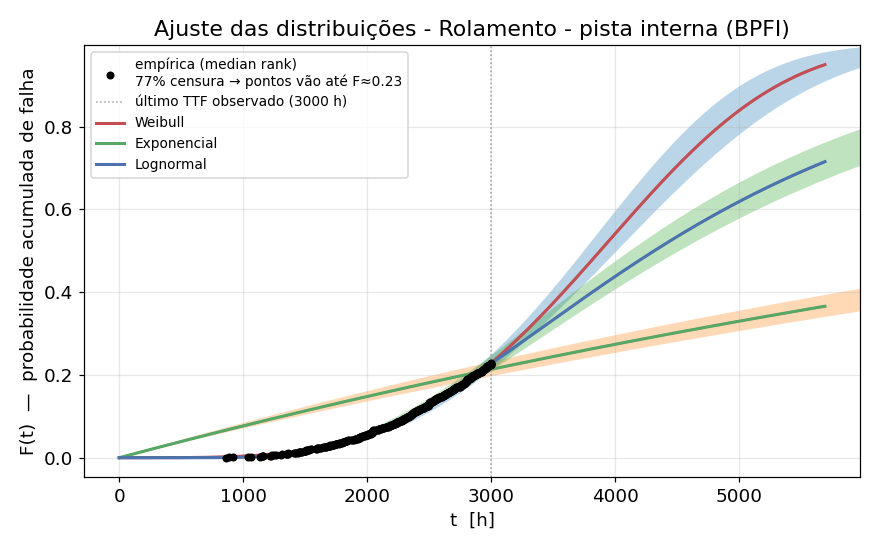
\includegraphics[width=\columnwidth]{p3_cdf_bpfi.png}
  \caption{Ajuste das distribuições sobre a CDF do rolamento BPFI. Os pontos
  pretos (empírica) terminam em F$\approx$0,23 porque 77\% das unidades
  simuladas foram censuradas à direita (não falharam até o horizonte de
  observação); os modelos extrapolam além desse ponto usando a informação das
  censuras. A Exponencial (verde) se afasta cedo pois assume falha imediata
  desde t=0, enquanto Weibull e Log-normal capturam o \textit{onset} tardio das
  falhas de desgaste. A linha pontilhada marca o último TTF observado (3000\,h).}
  \label{fig:cdf}
\end{figure}

\begin{figure}[!t]
  \centering
  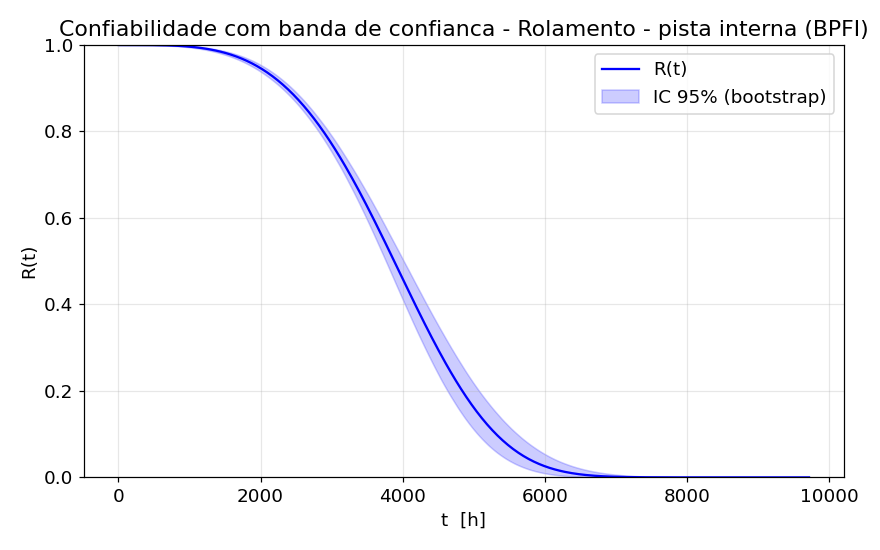
\includegraphics[width=\columnwidth]{p5_R_banda_bpfi.png}
  \caption{Confiabilidade $R(t)$ do rolamento BPFI com banda de confiança de
  95\% obtida por \textit{bootstrap} dos parâmetros da Weibull.}
  \label{fig:rbanda}
\end{figure}

\begin{figure}[!t]
  \centering
  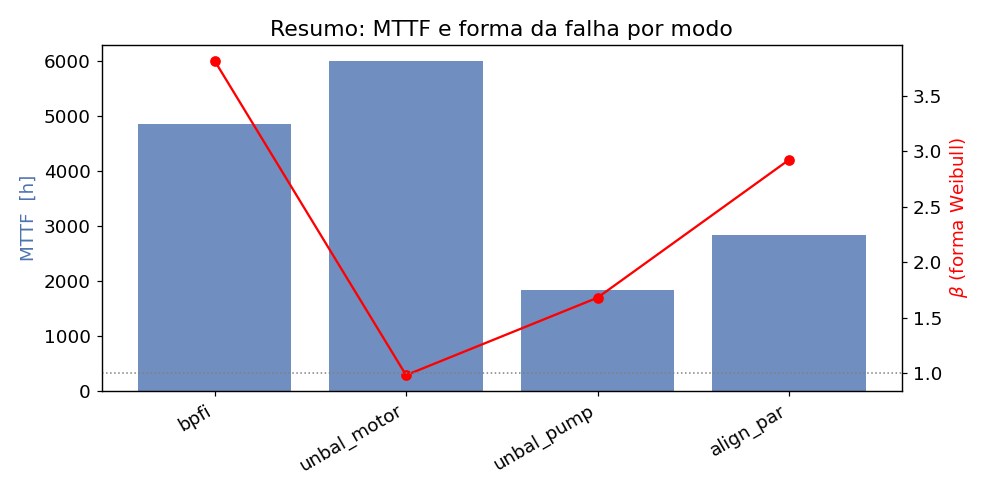
\includegraphics[width=\columnwidth]{resumo_modos.png}
  \caption{Resumo dos quatro modos com eixo Y duplo: MTTF em horas (barras azuis, referenciadas no eixo esquerdo) e parâmetro de forma $\beta$ da Weibull (linha vermelha com marcadores circulares, referenciada no eixo direito). A linha cinza pontilhada em $\beta=1$ demarca a transição entre falha por taxa constante e desgaste.}
  \label{fig:resumo}
\end{figure}

\begin{figure}[!t]
  \centering
  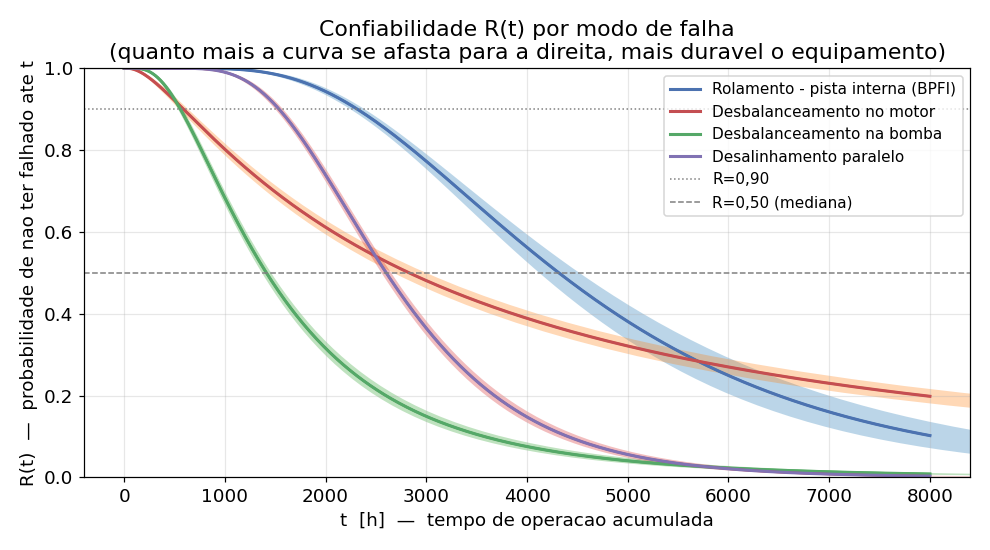
\includegraphics[width=\columnwidth]{comparacao_Rt_modos.png}
  \caption{Confiabilidade $R(t)$ dos quatro modos de falha: a curva mais à
  direita representa o modo mais durável. O desbalanceamento na bomba (verde)
  é o modo mais crítico --- metade das unidades falham antes de 1\,100\,h.
  O rolamento BPFI (azul) é o mais robusto, com MTTF de 4\,857\,h. As bandas
  coloridas são os IC\,95\% por \textit{bootstrap}.}
  \label{fig:rttodos}
\end{figure}

\begin{figure}[!t]
  \centering
  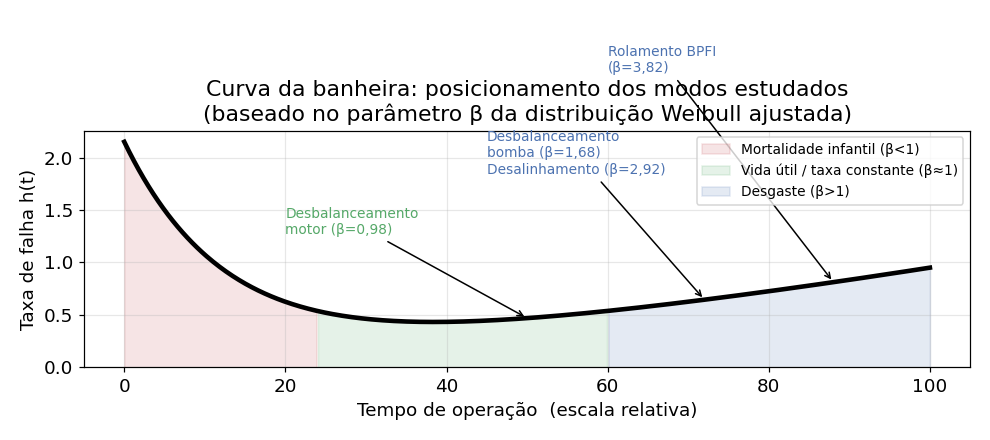
\includegraphics[width=\columnwidth]{curva_banheira.png}
  \caption{Curva da banheira com o posicionamento dos quatro modos segundo o parâmetro de forma $\beta$ da Weibull ajustada. A zona de mortalidade infantil ($\beta < 1$) não possui anotações pois nenhum modo mecânico progressivo se comporta como falha prematura de partida. O desbalanceamento no motor ($\beta\approx 1$) situa-se na vida útil (taxa de falha constante), enquanto os demais modos representam falhas de desgaste ($\beta > 1$).}
  \label{fig:banheira}
\end{figure}

\subsection{Sistema Motor-Bomba}
A Tabela~\ref{tab:sistema} e a Fig.~\ref{fig:sistema} apresentam o sistema, com
o desbalanceamento no motor representando o subsistema motor e o
desbalanceamento na bomba o subsistema bomba. A configuração série (real) tem
disponibilidade $0{,}983$ e confiabilidade na missão de 2000~h de apenas
$0{,}19$. As configurações redundantes elevam a disponibilidade a
$\approx 0{,}9997$ e a confiabilidade na missão a $0{,}35$ (paralelo) e $0{,}64$
(\textit{standby}).

Para série e paralelo, a disponibilidade estimada por Monte Carlo coincide com
a analítica até a terceira casa decimal (Fig.~\ref{fig:disp}), o que
valida a simulação: a coincidência é o resultado esperado, pois ambas as
estimativas modelam o mesmo processo de renovação. Para o \textit{standby} a
frio, a disponibilidade foi verificada apenas pela fórmula analítica (a barra
de Monte Carlo aparece como ``---'' na Tabela~\ref{tab:sistema}); isso ocorre
porque a simulação correta de uma reserva que não envelhece enquanto ociosa
exigiria modelar explicitamente o reparador e a fila de espera, o que foge ao
escopo deste trabalho.

\begin{table}[!t]
  \centering
  \caption{Sistema motor-bomba: disponibilidade e confiabilidade na missão
  (2000~h). Standby verificado apenas analiticamente.}
  \label{tab:sistema}
  \footnotesize
  \begin{tabular}{lccc}
    \toprule
    Configuração & $A$ (analítico) & $A$ (Monte Carlo) & $R(2000\,\mathrm{h})$ \\
    \midrule
    Série (real)        & 0,98316 & 0,98325 & 0,191 \\
    Paralelo (ativo)    & 0,99972 & 0,99976 & 0,348 \\
    \textit{Standby}    & 0,99970 & ---     & 0,642 \\
    \bottomrule
  \end{tabular}
\end{table}

\begin{figure}[!t]
  \centering
  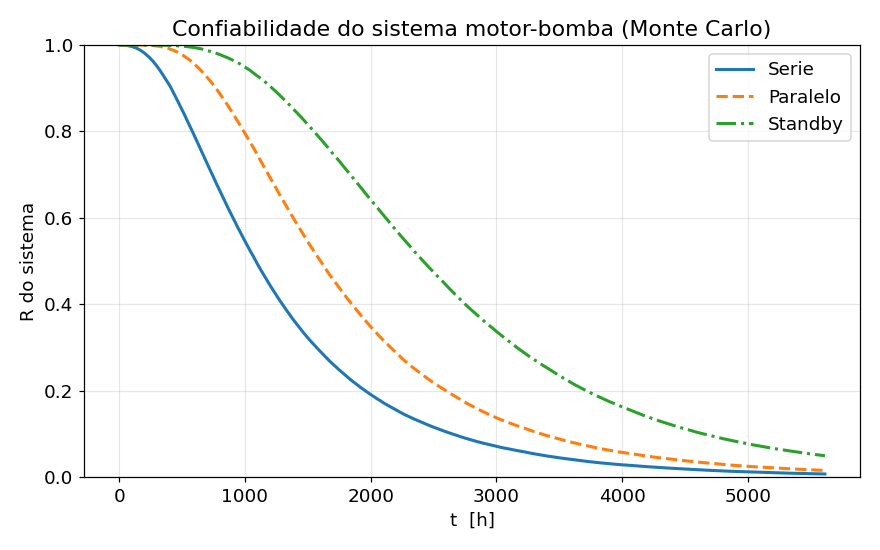
\includegraphics[width=\columnwidth]{p6_sistema_R.png}
  \caption{Confiabilidade $R(t)$ do sistema motor-bomba por Monte Carlo nas três
  configurações. A ordenação \textit{standby} $>$ paralelo $>$ série é a
  esperada.}
  \label{fig:sistema}
\end{figure}

\begin{figure}[!t]
  \centering
  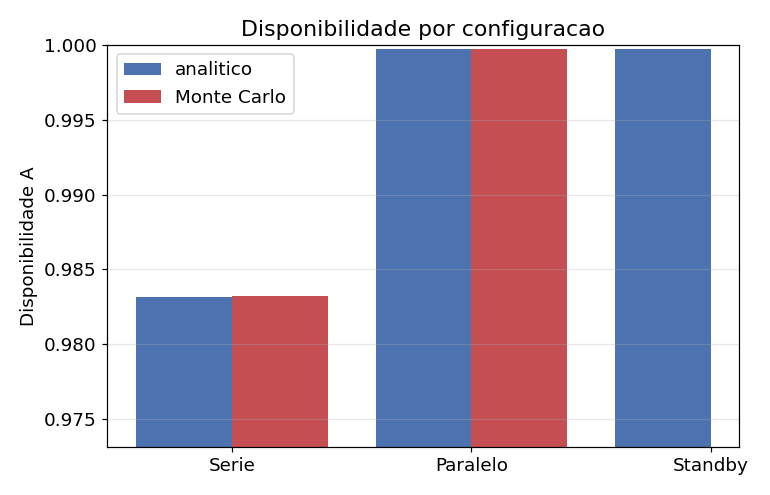
\includegraphics[width=\columnwidth]{p6_disponibilidade.png}
  \caption{Disponibilidade por configuração: comparação entre o valor analítico
  e a estimativa por Monte Carlo (coincidem para série e paralelo).}
  \label{fig:disp}
\end{figure}

% =========================================================================
% V. DISCUSSAO
% =========================================================================
\section{Discussão}
\label{sec:disc}

\subsection{Comparação com Referências}
A Tabela~\ref{tab:comparacao} confronta os resultados com faixas de referência.
Os parâmetros de forma situam-se na região de desgaste reportada para máquinas
rotativas ($\beta$ entre $1{,}5$ e $4$ para fadiga e
desgaste~\cite{oconnor2012}); o valor do rolamento ($\beta=3{,}82$) é alto em
relação à faixa típica de rolamentos ($1{,}5$--$2{,}0$), o que é atribuído à
dinâmica do modelo de degradação (a dispersão da vida é governada pelo
coeficiente $c$ da taxa) e não à fadiga intrínseca do rolamento. O limiar de
falha adotado, $L = \mu_0 + 0{,}5\,(D_{max}-\mu_0)$, coloca o ponto de falha
no meio do caminho entre a condição saudável e a severidade máxima observada;
a razão $L/\mu_0$ resultante varia entre $1{,}1\times$ (desbalanceamento na
bomba, onde $D_{max}$ é pouco maior que $\mu_0$) e $2{,}2\times$
(desalinhamento paralelo, onde $D_{max}\approx 3{,}3\,\mu_0$). A
ISO~20816-3~\cite{iso20816} define faixas de severidade de vibração para
máquinas rotativas (zonas~A a~D); a transição da zona~A (aceitável) para a
zona~C (alerta) corresponde a um aumento típico de $2$--$4\times$ na amplitude,
dependendo da classe da máquina. Assim, o limiar adotado situa-se em geral
abaixo da fronteira~C, o que equivale a declarar falha funcional ainda na
faixa de alerta --- uma escolha conservadora coerente com manutenção baseada
em condição. As disponibilidades de uma unidade ($0{,}987$--$0{,}995$) caem na
faixa usual de bombas industriais ($0{,}95$--$0{,}99$).

\begin{table}[!t]
  \centering
  \caption{Comparação com faixas de referência da literatura/normas.}
  \label{tab:comparacao}
  \footnotesize
  \begin{tabular}{lcc}
    \toprule
    Grandeza & Obtido & Referência \\
    \midrule
    $\beta$ rolamento          & 3,82 & 1,5--4,0 (desgaste)~\cite{oconnor2012} \\
    $\beta$ desbalanceamento   & 0,98 & $\approx 1$ (constante) \\
    $\beta$ desalinhamento     & 2,92 & $>1$ (desgaste) \\
    $A$ (uma unidade)          & 0,987--0,995 & 0,95--0,99 (bombas) \\
    Limiar ($L/\mu_0$)         & 1,1--2,2$\times$ & zona A$\to$C: 2--4$\times$,~ISO~20816~\cite{iso20816} \\
    \bottomrule
  \end{tabular}
\end{table}

\subsection{Premissas e Limitações}
Três pontos delimitam a interpretação. Primeiro, como o conjunto de dados é de
\textit{snapshots}, os TTF resultam de um modelo de degradação, não de falhas
observadas no tempo; a escala $\Delta\tau$ e a dispersão $c$ são premissas de
modelagem documentadas. Por isso, o MTTF aqui obtido ($1836$--$5997$~h) é o
tempo até a falha funcional condicionado a um defeito já em
desenvolvimento, e não o MTBF intrínseco do equipamento saudável (que, para
bombas, é da ordem de dezenas de milhares de horas); os dois não são
diretamente comparáveis. Segundo, a análise cobre quatro modos representativos
em uma velocidade cada, e não a totalidade das falhas, velocidades e
modalidades (corrente) do conjunto. Terceiro, a disponibilidade do
\textit{standby} foi verificada apenas analiticamente. Apesar disso, as
conclusões relativas --- ordenação dos modos por estágio de falha e ganho de
disponibilidade com redundância --- são robustas às premissas de escala.

% =========================================================================
% VI. CONCLUSAO
% =========================================================================
\section{Conclusão}

Demonstrou-se uma rota reprodutível para derivar indicadores clássicos de
confiabilidade a partir de sinais de vibração de um conjunto motor-bomba,
aplicando diretamente os métodos da disciplina: extração de séries de TTF com
censura, ajuste de distribuições de vida com seleção por AICc, intervalos de
confiança por \textit{bootstrap}, cálculo de $R(t)$, $h(t)$, MTTF e
disponibilidade, e simulação de Monte Carlo de um DBC. Os parâmetros de forma
obtidos são coerentes com a literatura de desgaste de máquinas rotativas, e a
disponibilidade de uma unidade cai nas faixas industriais usuais. A modelagem do
sistema mostra que adicionar uma unidade em paralelo ou em \textit{standby}
reduz a indisponibilidade de $\approx 1{,}7\%$ para $\approx 0{,}03\%$,
constituindo o principal argumento quantitativo para uma decisão de redundância.

Como trabalho futuro, sugere-se: estender a análise aos demais modos e às duas
modalidades de sensor (incluindo assinaturas de corrente para falhas elétricas);
substituir a premissa de escala severidade-tempo por dados de
\textit{run-to-failure} quando disponíveis; e acoplar o pipeline a um modelo de
predição de vida útil remanescente (RUL) para evoluir da manutenção baseada em
condição para a preditiva.

\smallskip
\noindent\textbf{Repositório:} código-fonte, figuras e documento em
\href{https://github.com/felcoslop/TP_CONFIABILIDADE}{\texttt{github.com/felcoslop/TP\_CONFIABILIDADE}}.

% =========================================================================
% REFERENCIAS
% =========================================================================
\begin{thebibliography}{99}

\bibitem{bruinsma2024}
S. Bruinsma, R.~D. Geertsma, R. Loendersloot, and T. Tinga,
``Motor current and vibration monitoring dataset for various faults in an
E-motor-driven centrifugal pump,''
\textit{Data in Brief}, vol.~52, art.~109987, Feb. 2024.
doi: \href{https://doi.org/10.1016/j.dib.2023.109987}{10.1016/j.dib.2023.109987}.
Conjunto de dados: \href{https://doi.org/10.4121/2b61183e-c14f-4131-829b-cc4822c369d0}{4TU.ResearchData}.

\bibitem{oconnor2012}
P.~D.~T. O'Connor and A. Kleyner,
\textit{Practical Reliability Engineering}, 5th~ed.
Chichester: Wiley, 2012.

\bibitem{meeker1998}
W.~Q. Meeker and L.~A. Escobar,
\textit{Statistical Methods for Reliability Data}.
New York: Wiley-Interscience, 1998.

\bibitem{colosimo2006}
E.~A. Colosimo and S.~R. Giolo,
\textit{Análise de Sobrevivência Aplicada}, 1ª~ed.
São Paulo: Blucher, 2006.

\bibitem{iso20816}
ISO, ``Mechanical vibration --- Measurement and evaluation of machine vibration
--- Part~3,'' \textit{ISO~20816-3:2022}, Geneva, 2022.

\bibitem{robert2010}
C.~P. Robert and G. Casella,
\textit{Introducing Monte Carlo Methods with R}.
New York: Springer, 2010.

\bibitem{zio2013}
E. Zio,
\textit{The Monte Carlo Simulation Method for System Reliability and Risk
Analysis}. London: Springer, 2013.

\bibitem{reid2022}
M. Reid, ``\textit{reliability} --- a Python library for reliability
engineering,'' Zenodo, 2024.
doi: \href{https://doi.org/10.5281/zenodo.3938000}{10.5281/zenodo.3938000}.

\bibitem{bessani2026}
M. Bessani,
``Notas de aula e \textit{scripts} da disciplina EEE017 -- Confiabilidade de
Sistemas,'' UFMG, Belo Horizonte, 2026.

\end{thebibliography}

\end{document}
